\newpage
\section{Preprocesing}

Preprocesing to proces przygotowywania danych wejściowych tak by nadawały się do szkolenia sieci.

\subsection{Teoria}

Proces preprocesingu dzieli się na trzy etapy.
\begin{enumerate}
	\item Redukcja alfabetu (mapowanie znaków)
	\item Zamiana zredukowanych tekstów na tensory
	\item Podział tensorów na batche
\end{enumerate}

Należy przy tym dodać że domyślnie dostępnymi językami w bibliotece są:
\languages 


\subsubsection{Redukcja alfabetu}
Redukcja alfabetu to sprytny sposób zmniejszenia liczby znaków w alfabecie, tak by uczenie sieci było
efektywniejsze. Możemy definiować nasze własne 'mappery'. Przykładowy fragment pliku do redukcji alfabetu języka
angielskiego znajduje się poniżej (został on znacznie skrócony wzlgędem oryginału żeby zachować lepszą
czytelność)

\begin{python}
charmap = {
    u' ': u' ',                 # kept Zs (92447)
    u'e': u'e',
    u't': u't',
    u'o': u'o',
    u'a': u'a',
    u'n': u'n',
    u'i': u'i',
    u's': u's',
    u'h': u'h',
    u'r': u'r',
    u'\n': u'\n',               # kept Cc (13082)
    u'l': u'l',
    u'd': u'd',
    u'u': u'u',
    u'y': u'y',
    u'm': u'm',
    u'g': u'g',
    u'w': u'w',
    u',': u',',                 # kept Po (5250)
    u"'": "'",                  # single quote
    u'.': u'.',                 # kept Po (4826)
    u'f': u'f',
    u'c': u'c',
    u'b': u'b',
    u'p': u'p',
    u'-': u'-',                 # kept Pd (3253)
    u'k': u'k',
    u'I': u'\xb9i',             # decomposed caps
    u'v': u'v',
}
\end{python}

Tak przygotowany 'mapper' pozwala na zamiane wybranych znaków, które nie są kluczowe w procesie 
szkolenia sieci na wybrane, inne znaki.

\newpage
\subsubsection{Zamiana tekstów na tensory}
Aby zamienić teksty na tensory potrzebny jest nam alfabet. Alfabet definiujemy jako listę, której 
elementy są znakami. Tak wygląda fragment alfabetu z języka angielskiego:
\begin{python}
alphabet = [
    ' ',
    'e',
    't',
    'o',
    'a',
    'n',
    'i',
    's',
    'h',
    'r',  # 10
    '\\n',
    'l',
    'd',
    'u',
    'y',
    'm',
    'g',
    'w',
    ',',
    "'",  # 20
    '.',
    'f',
    'c',
    'b',
]
\end{python}

Każdy znak zredukowanego pliku wejściowego zamieniany jest na wektor wykorzystując alfabet, 
a wektory 'umieszczane' są w tensorze. Wykorzystywane przy tym jest \texttt{one hot encoding}.
Zamianę liter na wektory najłatwiej pokazać na przykładzie.

Załóżmy że nasz alfabet wygląda następująco:

\begin{python}
alphabet = [
    'a',  #0
    'b',  #1
    'c',  #2
    'd',  #3
 ]
\end{python} 
Jeśli zamienimy literę 'a' na wektor otrzymamy: 
 
\vspace{2mm}
$
\begin{bmatrix} 
1, & 0, & 0, & 0
\end{bmatrix} 
$
\vspace{2mm}

Ponieważ litera 'a' jest na pozycji 0 w alfabecie liczba 1 pojawiła się na pozycji 0 w wektorze.
Długość wektora wynosi 4 ponieważ tyle znaków znajduje się w alfabecie. A więc dla litery 
'c' wektor wyglądałby w następujący sposób:

\vspace{2mm}
$
\begin{bmatrix} 
0, & 0, & 1, & 0
\end{bmatrix} 
$
\vspace{2mm}

W ten sposób konwertowane są wszystkie znaki w plikach, które następnie umieszczane są w tensorze.
Tensor na tym etapie jest tablicą jednowymiarową, w którym znajdują się teksty tylko jednego autora, 
a elementami są wyżej wspomniane wektory umieszczane tam zgodnie z kolejnością ich występowania w tekście. 
Następnie następuje podział na batche.

\subsubsection{Rozdzielenie tensorów na paczki}
Jednym ze sposobów przyspieszenia czasu uczenia jest podzielenie danych na paczki (ang. batche).
Pozwala nam to na wykonywanie obliczeń na wielu danych jednocześnie. Poniżej przedstawiamy batchowanie
na przykładzie, dla którego przyjmiemy następujące założenia: 
\begin{itemize}
	\item rozmiar batcha równy 3
	\item liczba timestepów równa 3
	\item liczba autorów równa 4
	\item alfabet $\{a,b,c,d\}$
\end{itemize}

Każdy z autorów ma przyporządkowane nastpujące teksty:
\begin{itemize}
	\item autor 1: ``abacd''
	\item autor 2: ``dbaa''
	\item autor 3: ``cadb''
	\item autor 4: ``cbbcc''
\end{itemize}

Zamieniamy litery na wektory wedle wcześniejszego opisu, gdzie:
\vspace{3mm}
\newline 
$
a =
\begin{bmatrix} 
1, & 0, & 0, & 0
\end{bmatrix} 
$
\vspace{3mm}
\newline
$
b = 
\begin{bmatrix} 
0, & 1, & 0, & 0
\end{bmatrix} 
$
\vspace{3mm}
\newline 
$
c =
\begin{bmatrix} 
0, & 0, & 1, & 0
\end{bmatrix} 
$
\vspace{3mm}
\newline 
$
d =
\begin{bmatrix} 
0, & 0, & 0, & 1
\end{bmatrix} 
$
\vspace{1mm}
\newline 

Wektory umieszczamy w tensorach. Dla każdego autora przewidziany jest osobny tensor. 
Przykładowo dla autora 3 wyglądałby on następująco:
\vspace{3mm}

$
\begin{bmatrix} \begin{bmatrix} 0, & 0, & 1, & 0\end{bmatrix},  & \begin{bmatrix} 1, & 0, & 0, & 0\end{bmatrix}, & \begin{bmatrix} 0, & 0, & 0, & 1\end{bmatrix}, & \begin{bmatrix} 0, & 1, & 0, & 0\end{bmatrix} \end{bmatrix}
$



\begin{wrapfigure}{r}{0.6\textwidth}
\vspace{-4mm}
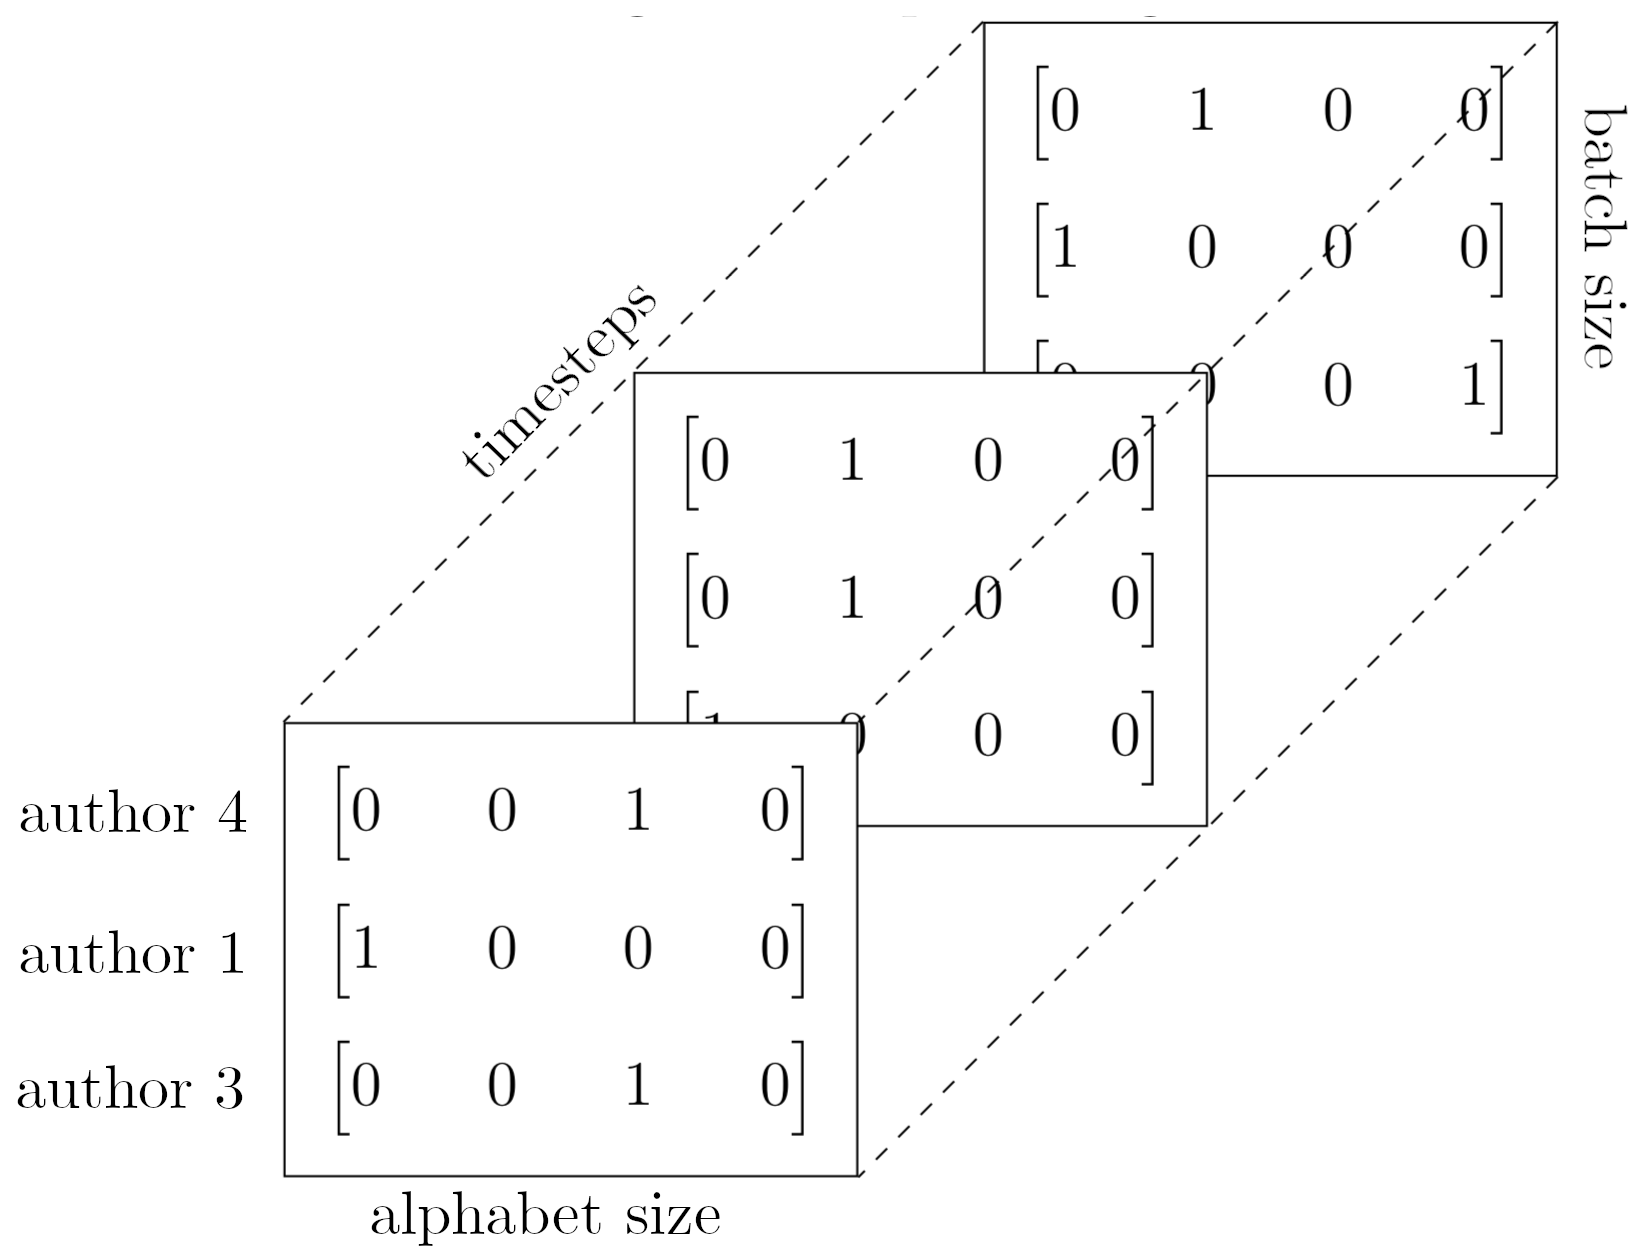
\includegraphics[width=\linewidth]{./images/batch.png}
\caption{Wizualizacja pierwszego batcha}
\label{fig:test2}
\vspace{-4mm}
\end{wrapfigure}
 
Następnie ze wszystkich tych tensorów tworzymy batche.
Dla tego przykładu każdy z batchy będzie tensorem o wymiarach 3 x 4 x 3 (rozmiar batcha $x$ rozmiar 
alfabetu $x$ ilość timestepów).
Do każdej takiej paczki będziemy losować autorów oraz ich kolejność. Załóżmy, że do pierwszego batcha
wylosowaliśmy autora 4, 1 oraz 3. Oznacza to, że w pierwszym timestepie w tensorze zawarta będzie 
patrząc ``od góry'': pierwsza litera autora 4, pierwsza litera autora 1 oraz pierwsza litera autora 3.
To ustawienie autorów w tensorach będzie już zawsze zachowane dla wszystkich timestepów w tym batchu. 
A więc dla drugiego timestepu będzie to: druga litera autora 4, druga litera autora 1 oraz druga 
litera autora 3. Dla trzeciego timestepu analogicznie. 

Może się zdarzyć sytuacja, że do batcha wylosowano dwa razy tego samego autora. Na przykład wylosowano
autorów 1 oraz 3, w kolejności: autor pierwszy, następnie znowu autor pierwszy, na końcu autor trzeci.
Dla identycznych założeń jak we wcześniejszym przykładzie w pierwszym batchu w pierwszym timestepie wyglądałoby to
 następująco: pierwsza litera autora 1, następnie pierwsza litera autora 1,
na końcu pierwsza litera autora 3. W drugim timestepie byłoby to:
druga litera autora 1, druga litera autora 1 oraz druga litera autora 3, itd.

Ilość batchy jest zależna od długości tekstów. 

\newpage
\subsection{Pliki wejściowe oraz wyjściowe}
Aby korzystać z modułu preprocessingu należy zachować określoną konwencję danych wejściowych. 

\subsubsection{Struktura wejścia}

\begin{enumerate}
	\item Wszystkie pliki tekstowe muszą być w formacie txt,
	\item folder z danymi wejściwoymi musi mieć konkretną strukture. W folderze każdego autora
		  powinny znajdować się jego teksty: 
			\begin{itemize}
				\item known$X$.txt gdzie $X$ jest numerem tekstu, tekstów known.txt może być wiele.
				\item unknown.txt
			\end{itemize}
\end{enumerate}

Przykład: 

\myspace
\dirtree{%
.1 data.
.2 authors.
.3 EN001.
.4 known01.txt.
.4 unknown.txt.
.3 EN002.
.4 known01.txt.
.4 known02.txt.
.4 known03.txt.
.4 unknown.txt.
.3 EN003.
.4 known01.txt.
.4 unknown.txt.
.3 EN004.
.4 known01.txt.
.4 known01.txt.
.4 unknown.txt.
.3 EN005.
.4 known01.txt.
.4 unknown.txt.
}
\myspace

\newpage
\subsubsection{Struktura wyjścia}

Wszystkie pliki wejściowe są zamieniane na tensory i dzielone na batche. Wszystkie pliki knownX.txt 
danego autora są wcześniej łączone w jeden plik, który później staje się tensorem. W ten sposób 
otrzymujemy następująco wyglądający folder wyjściowy, gdzie każdy plik EN$X$.pt (gdzie $X$ to numer)
 jest tensorem:

\myspace
\dirtree{%
.1 tensors.
.2 known.
.3 EN001.
.4 EN001.pt.
.3 EN002.
.4 EN002.pt.
.3 EN003.
.4 EN003.pt.
.3 EN004.
.4 EN004.pt.
.3 EN005.
.4 EN005.pt.
.2 unknown.
.3 EN001.
.4 EN001.pt.
.3 EN002.
.4 EN002.pt.
.3 EN003.
.4 EN003.pt.
.3 EN004.
.4 EN004.pt.
.3 EN005.
.4 EN005.pt.
}
\myspace
